\chapter{Application to compact finite difference evaluation}

\section{Compact finite difference evaluation on parallel systems}

Because of the high computational cost
and memory requirements of direct numerical simulation,
parallelism is mandatory.
The computation of derivatives using
compact finite differences involves two primary steps:

\begin{enumerate}
\item The evaluation of the right hand sides
    of Eq. (\ref{eqn:general-compact})
    at each grid point.
\item The solution of the tridiagonal system
    [Eq. (\ref{eqn:general-compact})]
    for each line of grid points.
\end{enumerate}

Both of these operations are amenable to parallel operations.
The right hand side calculation is a pointwise
\emph{stencil} operation, i.e.,
at every point in the domain,
the value of the right hand side
is computed as a combination of function values
at that point and its neighbouring points.
The stencil operations at individual points
are independent,
making the overall calculation highly parallelizable.
The solution of the tridiagonal systems,
is of course parallelizable
as has been discussed in previous sections.

Without loss of generality,
we consider the parallelization of
compact finite difference evaluations for 2-dimensional problems.
We assume that the derivative is being calulated
for the coordinate direction along which
elements are stored contiguously in memory, i.e.,
the ``fastest'' coordinate direction.

\subsection{Single GPU}

\begin{figure}
\begin{center}
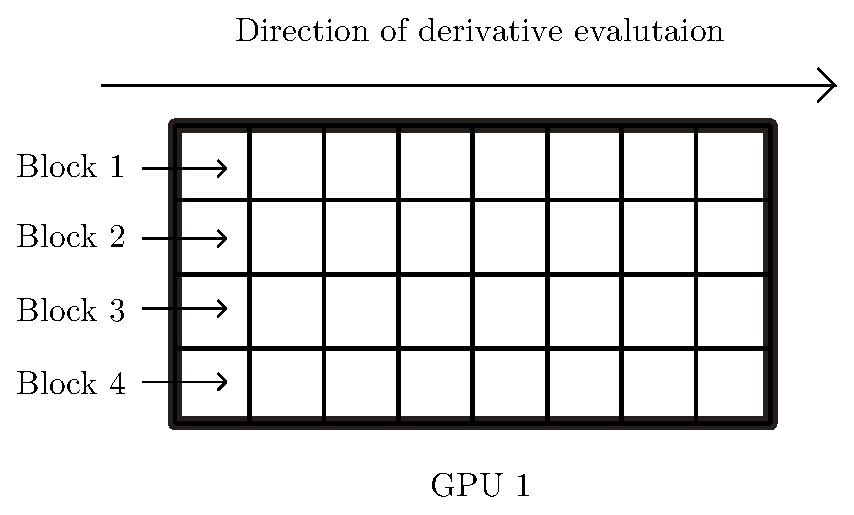
\includegraphics[height=150pt]{img/compact-single-gpu.eps}
\caption{Computational domain in 3-D.}
\label{fig:compact-single-gpu}
\end{center}
\end{figure}

For a single GPU \ref{fig:compact-single-gpu},
when calculating the right hand sides,
each point in the grid is mapped to a single thread,
and each thread applies the required stencil operation
to compute the right hand side at that point.
We note that threads near the left and right boundaries
apply a different stencil from the interior threads.
The implementation of GPU kernels for
stencil operations such as these is a topic of wide study.
The most important considerations were brought out
in the paper by Micikevicius et al. ~\ref{micikevicius20093d}.
For solving the tridiagonal systems,
each thread block of the GPU is mapped to a
different \emph{grid line}
aligned along the
direction the derivatives are being calculated.
The right hand sides are stored
contiguously along these grid lines
(as in Fig. \ref{fig:block-mapping}),
and the modified cyclic reduction algorithm developed
can be used to solve for the derivatives.

\subsection{Multiple GPUs on a single node}

\begin{figure}
\begin{center}
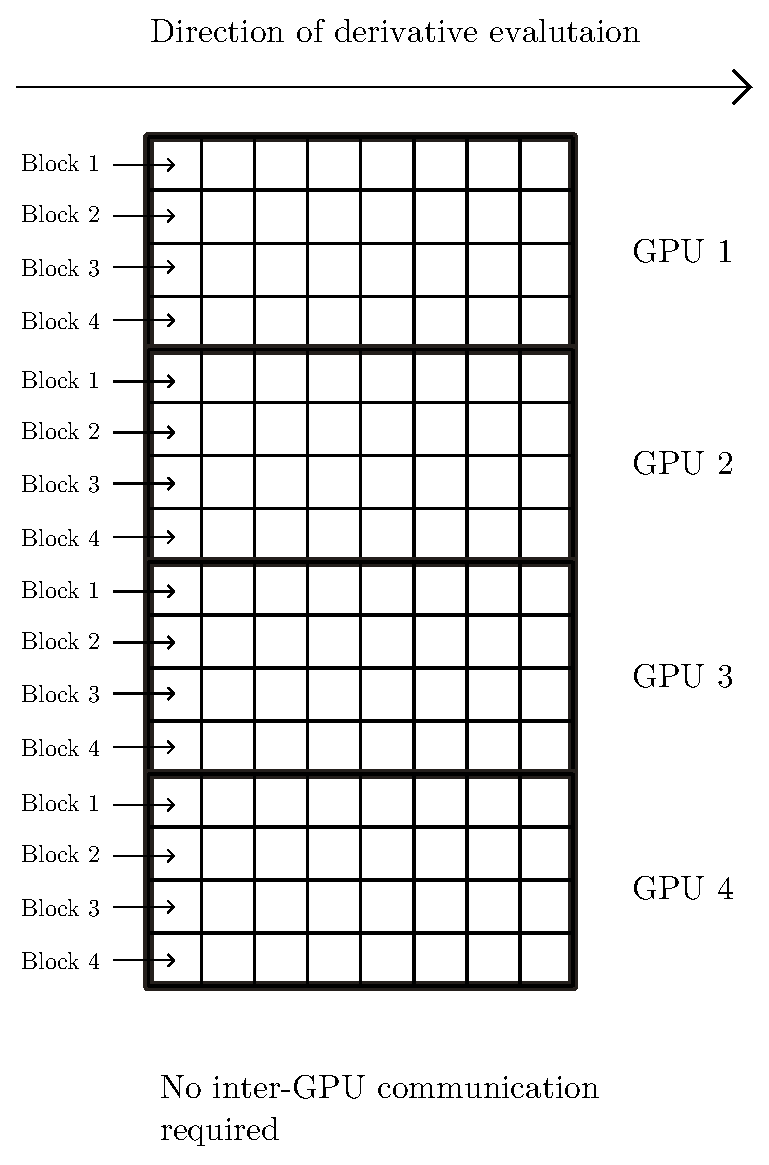
\includegraphics[width=250pt]{img/compact-shared-gpu.eps}
\caption{Compact finite differences - multiple GPUs
    on same node}
\label{fig:compact-shared-gpu}
\end{center}
\end{figure}

Here, we consider the case of multiple GPUs
on a single shared memory node, i.e.,
multiple GPUs attached to the same PCI-e bus.
In this case, every GPU is visible to the host,
and the GPUs read from and write into
the same host memory space.
The domain is divided into a number of
into ``subdomains'',
as shown in \ref{fig:compact-shared-gpu}.
The domain decomposition is done such that
only a single subdomain is used along the
coordinate direction of the derivatives.
This is the method presented by
Sakharnykh et al. ~\cite{sakharnykhADIconf},
and it has the advantage that
no coordination between GPUs is required:
each GPU is assigned an independent
set of grid lines to solve.

\subsection{Distributed GPUs - restricted in one direction}

\begin{figure}
\begin{center}
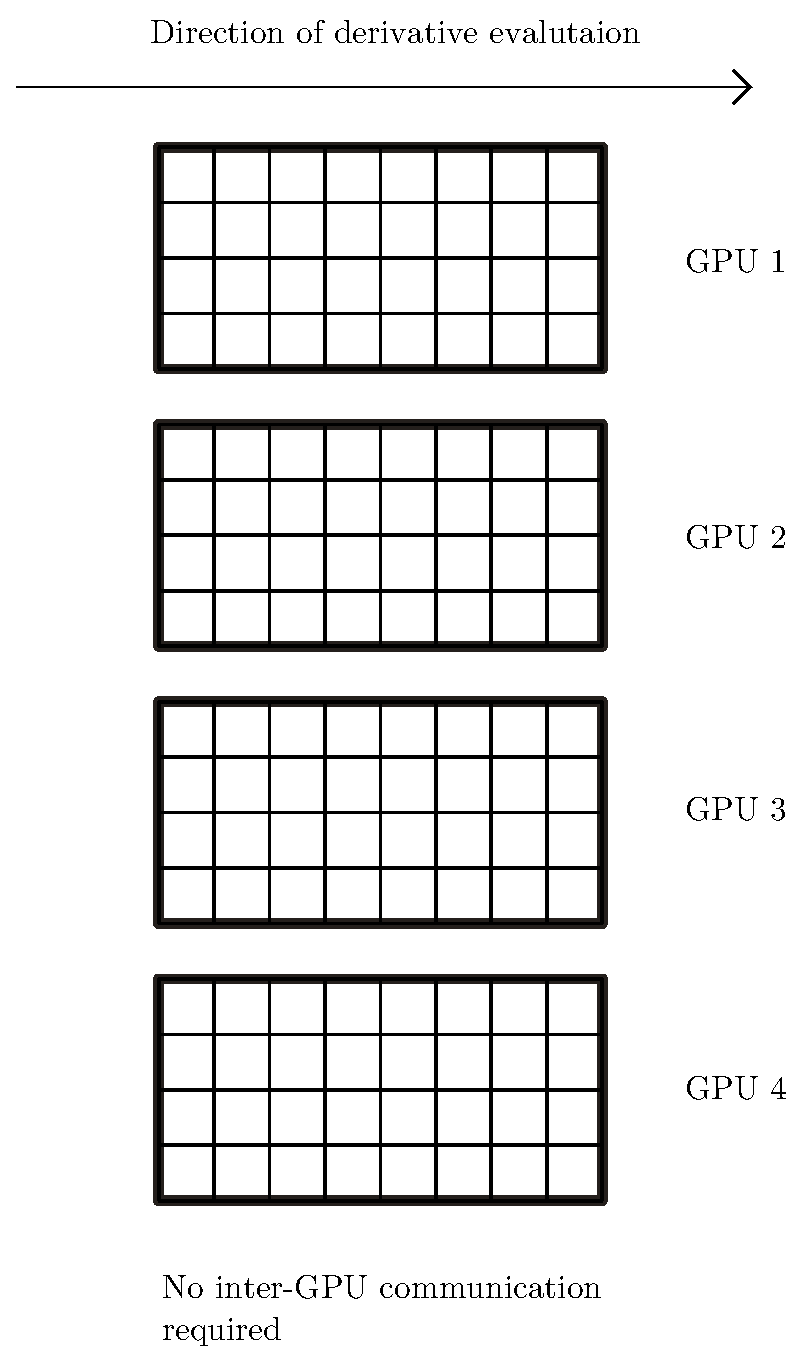
\includegraphics[width=200pt]{img/compact-distributed-restricted.eps}
\caption{Compact finite differences - distributed GPUs and
    restriced in one direction}
\label{fig:compact-distributed-restricted}
\end{center}
\end{figure}

For larger problems,
a distributed system may be required.
Here, the simplest strategy is to use a domain decomposition
as shown in \ref{fig:compact-distributed-restricted}.
Here again, 
no inter-GPU communication is required.
By restricting the distribution along one coordinate direction,
the ease of solution of the tridaigonal systems is maintained.

\subsection{Distributed GPUs in all directions}

\begin{figure}
\begin{center}
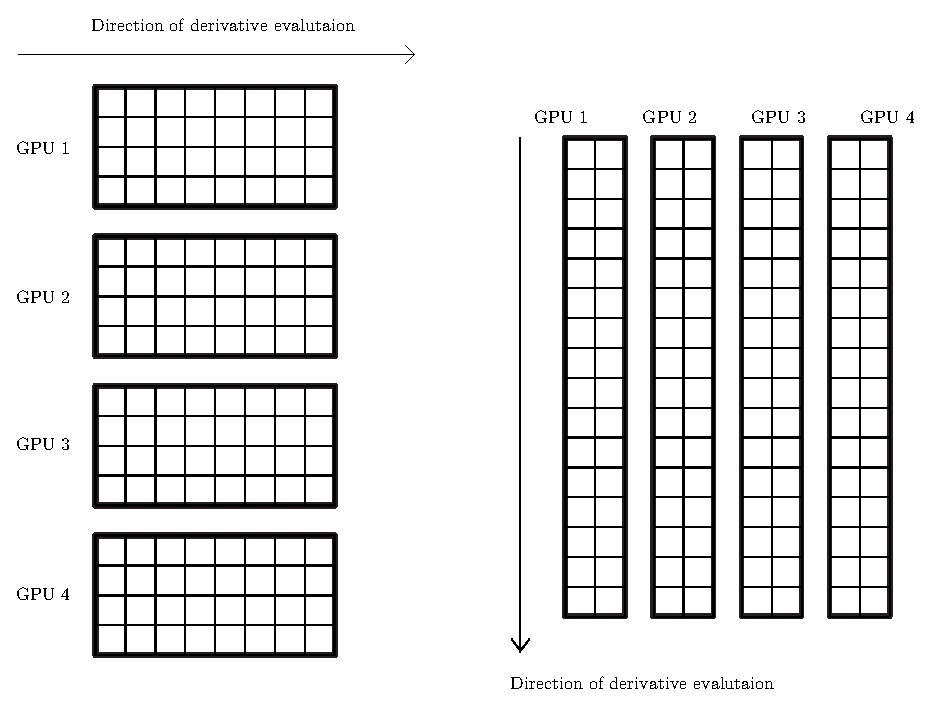
\includegraphics[height=250pt]{img/compact-restricted-transpose.eps}
\caption{Compact finite difference evaluation in both coordinate directions}
\label{fig:compact-restricted-transpose}
\end{center}
\end{figure}

The above domain decomposition strategies are convenient,
but can be impractical for some cases.
For instance,
let us consider the evaluation of derivatives
in the other coordinate direction
(Fig. \ref{fig:compact-restricted-transpose}).
Because the grid lines aligned along this direction
must reside on the same GPU,
it follows that:
%
\begin{enumerate}
    \item A \emph{global} transposition or rearrangement
        of the data is required,
        such that each GPU now contains data for
        grid lines aligned in the direction orthogonal
        to the previous direction.
        For distributed systems,
        this transposition can be an extremely expensive process.
    
    \item For domains that are much longer along one coordinate
        direction compared to the other(s),
        the subdomains may become impractically \emph{slender}.
\end{enumerate}
%
Such decomposition strategies are therefore, generally applicable
when compact finite difference schemes are used only
in a single direction.
For the other coordinate directions,
explicit finite difference schemes may be used,
which has the disadvantages discussed earlier.
To accomodate compact finite difference schemes in all the coordinate
directions,
the domain decomposition generally must be performed in all directions,
as shown in \ref{fig:compact-distributed-all}.

\begin{figure}
\begin{center}
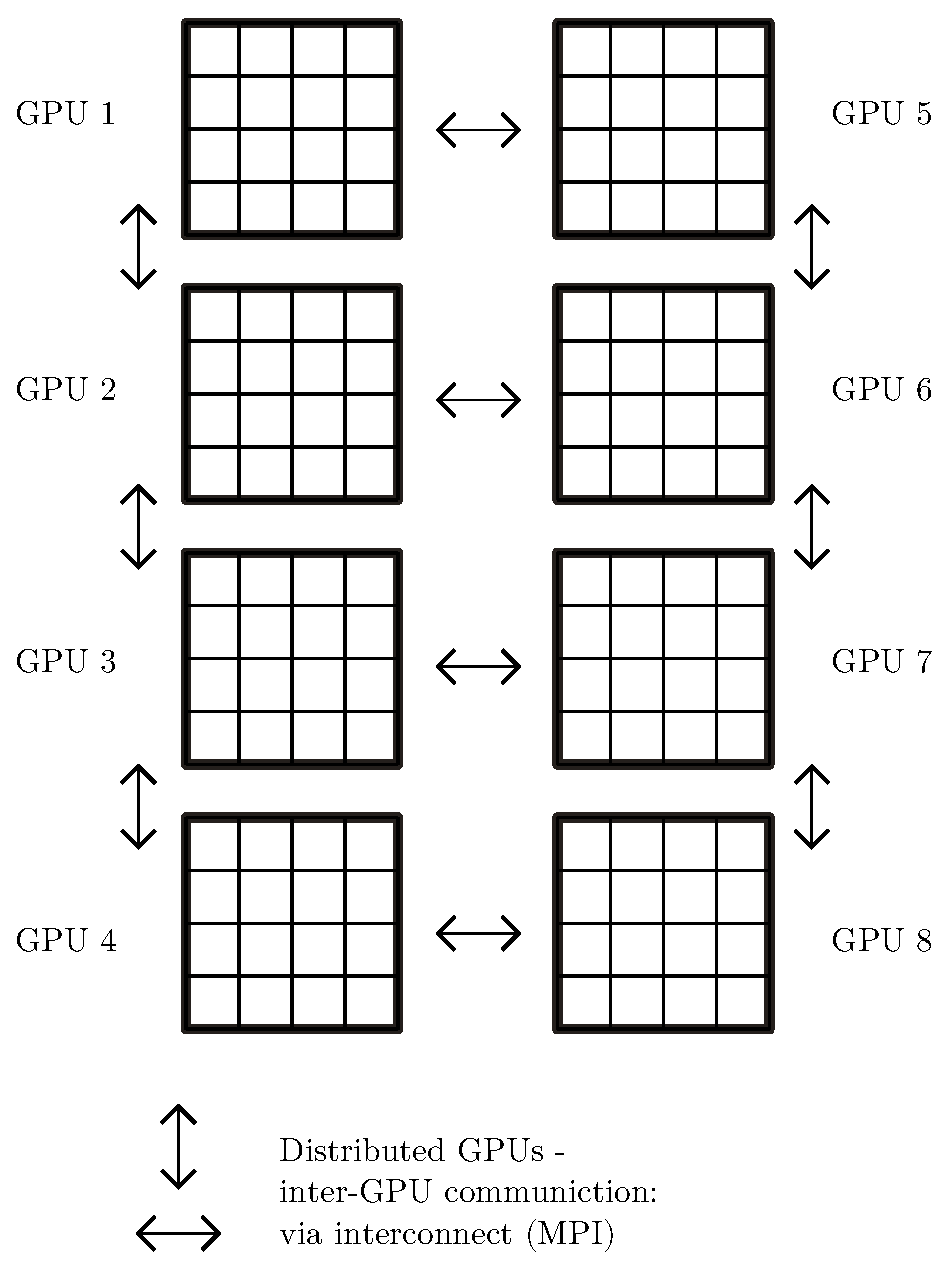
\includegraphics[width=200pt]{img/compact-distributed-all.eps}
\caption{Compact finite differences - distributed GPUs in all
    directions}
\label{fig:compact-distributed-all}
\end{center}
\end{figure}

\section{Distributed tridiagonal solver}

\begin{figure}
\begin{center}
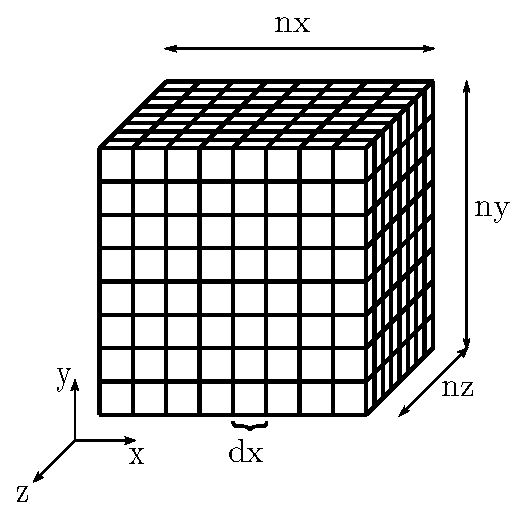
\includegraphics[height=150pt]{img/computational-domain.eps}
\caption{Computational domain in 3-D.}
\label{fig:computational-domain}
\end{center}
\end{figure}
%
The computational domain considered
is a 3-dimensional,
regular, Cartesian grid with
$nx$, $ny$ and $nz$ grid points and grid spacing of
$dx$, $dy$ and $dz$ in the
respective coordinate directions,
\ref{fig:computational-domain},
Structured grids such as these
are widely used in DNS because they lend themselves naturally
to finite-difference methods.



    \subsection{General algorithm}

    Algorithm by Mattor et al.

    \subsection{Specialization for compact finite difference
        evaluations}

    Right hand side evaluation
    

\section{GPU application}

    \subsection{GPU-GPU communication}
        \subsubsection{Naive strategy}
        
        GPU-CPU-CPU-GPU
        
        \subsubsection{NVIDIA GPUDirect Technology}

        GPU-GPU

    \subsection{Implementation}
        \subsubsection{Precomputing coefficients}
        
        Recognize the coefficients of the
        local tridiagonal system

        \subsubsection{Solving secondary systems}

        The computation is offline,
        solve only one system
        Move results to GPU

        \subsubsection{Computing right hand sides}
    
        Stencil code
        Show the halo swapping strategy

        \subsubsection{Solving primary systems}

        Each of the systems is solved using the NEATO algorithm

        \subsubsection{Constructing and solving reduced systems}
        
        Interleaved tridagonal systems,
        solved using a p-Thomas strategy (reference?)

        \subsubsection{Summing primary and secondary solutions}
        
        Completely pointwise
        
        \subsubsection{Evaluating derivatives in other
            coordinate directions}

        Permutation kernels
